\documentclass[twoside]{book}

% Packages required by doxygen
\usepackage{calc}
\usepackage{doxygen}
\usepackage{graphicx}
\usepackage[utf8]{inputenc}
\usepackage{makeidx}
\usepackage{multicol}
\usepackage{multirow}
\usepackage{textcomp}
\usepackage[table]{xcolor}

% Font selection
\usepackage[T1]{fontenc}
\usepackage{mathptmx}
\usepackage[scaled=.90]{helvet}
\usepackage{courier}
\usepackage{amssymb}
\usepackage{sectsty}
\renewcommand{\familydefault}{\sfdefault}
\allsectionsfont{%
  \fontseries{bc}\selectfont%
  \color{darkgray}%
}
\renewcommand{\DoxyLabelFont}{%
  \fontseries{bc}\selectfont%
  \color{darkgray}%
}

% Page & text layout
\usepackage{geometry}
\geometry{%
  a4paper,%
  top=2.5cm,%
  bottom=2.5cm,%
  left=2.5cm,%
  right=2.5cm%
}
\tolerance=750
\hfuzz=15pt
\hbadness=750
\setlength{\emergencystretch}{15pt}
\setlength{\parindent}{0cm}
\setlength{\parskip}{0.2cm}
\makeatletter
\renewcommand{\paragraph}{%
  \@startsection{paragraph}{4}{0ex}{-1.0ex}{1.0ex}{%
    \normalfont\normalsize\bfseries\SS@parafont%
  }%
}
\renewcommand{\subparagraph}{%
  \@startsection{subparagraph}{5}{0ex}{-1.0ex}{1.0ex}{%
    \normalfont\normalsize\bfseries\SS@subparafont%
  }%
}
\makeatother

% Headers & footers
\usepackage{fancyhdr}
\pagestyle{fancyplain}
\fancyhead[LE]{\fancyplain{}{\bfseries\thepage}}
\fancyhead[CE]{\fancyplain{}{}}
\fancyhead[RE]{\fancyplain{}{\bfseries\leftmark}}
\fancyhead[LO]{\fancyplain{}{\bfseries\rightmark}}
\fancyhead[CO]{\fancyplain{}{}}
\fancyhead[RO]{\fancyplain{}{\bfseries\thepage}}
\fancyfoot[LE]{\fancyplain{}{}}
\fancyfoot[CE]{\fancyplain{}{}}
\fancyfoot[RE]{\fancyplain{}{\bfseries\scriptsize Generated on Thu May 22 2014 01\-:23\-:54 for Simplex by Doxygen }}
\fancyfoot[LO]{\fancyplain{}{\bfseries\scriptsize Generated on Thu May 22 2014 01\-:23\-:54 for Simplex by Doxygen }}
\fancyfoot[CO]{\fancyplain{}{}}
\fancyfoot[RO]{\fancyplain{}{}}
\renewcommand{\footrulewidth}{0.4pt}
\renewcommand{\chaptermark}[1]{%
  \markboth{#1}{}%
}
\renewcommand{\sectionmark}[1]{%
  \markright{\thesection\ #1}%
}

% Indices & bibliography
\usepackage{natbib}
\usepackage[titles]{tocloft}
\setcounter{tocdepth}{3}
\setcounter{secnumdepth}{5}
\makeindex

% Hyperlinks (required, but should be loaded last)
\usepackage{ifpdf}
\ifpdf
  \usepackage[pdftex,pagebackref=true]{hyperref}
\else
  \usepackage[ps2pdf,pagebackref=true]{hyperref}
\fi
\hypersetup{%
  colorlinks=true,%
  linkcolor=blue,%
  citecolor=blue,%
  unicode%
}

% Custom commands
\newcommand{\clearemptydoublepage}{%
  \newpage{\pagestyle{empty}\cleardoublepage}%
}


%===== C O N T E N T S =====

\begin{document}

% Titlepage & ToC
\hypersetup{pageanchor=false}
\pagenumbering{roman}
\begin{titlepage}
\vspace*{7cm}
\begin{center}%
{\Large Simplex \\[1ex]\large 0.\-5 }\\
\vspace*{1cm}
{\large Generated by Doxygen 1.8.6}\\
\vspace*{0.5cm}
{\small Thu May 22 2014 01:23:54}\\
\end{center}
\end{titlepage}
\clearemptydoublepage
\tableofcontents
\clearemptydoublepage
\pagenumbering{arabic}
\hypersetup{pageanchor=true}

%--- Begin generated contents ---
\chapter{Simplex}
\label{index}\hypertarget{index}{}\begin{DoxyAuthor}{Author}
Pawel Zurek 
\end{DoxyAuthor}
\begin{DoxyDate}{Date}
16.\-03.\-2014 
\end{DoxyDate}
\begin{DoxyVersion}{Version}
1.\-1.\-b
\end{DoxyVersion}
Program umożliwia liczenie czasu trwania operacji wypelniania liczbami stosu / kolejki.\hypertarget{index_etykieta-wazne-cechy}{}\section{Najważniejsze cechy}\label{index_etykieta-wazne-cechy}
Program sluzy do liczenia czasu wypelnienia liczbami stosow i kolejek za pomoca \-:\par


\par
-\/$>$ list \par
-\/$>$ tablic ( po przekroczeniu rozmiaru tablicy, rozmiar powiekszany o jeden ) \par
-\/$>$ tablic ( po przekroczeniu rozmiaru tablicy, rozmiar zwiekszany dwukrotnie )\hypertarget{index_etykieta-op-algorytm}{}\section{Opis algorytmu}\label{index_etykieta-op-algorytm}
Algorytm w tym zadaniu to 6 petli \-: \par
-\/$>$ wypelnienie stosu za pomoca listy \par
-\/$>$ wypelnienie kolejki za pomoca listy \par
-\/$>$ wypelnienie stosu za pomoca tablicy ( rozmiar o jeden ) \par
-\/$>$ wypelnienie stosu za pomoca tablicy ( rozmiar x2 ) \par
-\/$>$ wypelnienie kolejki za pomoca tablicy ( rozmiar o jeden ) \par
-\/$>$ wypelnienie kolejki za pomoca tablicy ( rozmiar x2)

\par
,na ktora sklada sie wypelnienie nastepujaca iloscia elementow\-:

\par
-\/$>$ 10 \par
-\/$>$ 100 \par
-\/$>$ 1000 \par
-\/$>$ 10000

Czasy sa wyprowadzane na standartowe wyjscie. 
\chapter{Class Index}
\section{Class List}
Here are the classes, structs, unions and interfaces with brief descriptions\-:\begin{DoxyCompactList}
\item\contentsline{section}{\hyperlink{class_graf}{Graf} \\*Modeluje pojecie graf. Klasa sluzy glownie do wykonania algorytmu wyszukiwania, czyli znalezienia polaczenia miedzy dwoma punktami }{\pageref{class_graf}}{}
\item\contentsline{section}{\hyperlink{structpor}{por} \\*Struktura porownywania Struktura ta ma na celu ulatwienie dzialania algorytmu wyszukiwania ( Dijkstry ) Prownuje ona wartosci drogi miedzy dwoma wezlami }{\pageref{structpor}}{}
\item\contentsline{section}{\hyperlink{struct_wezel}{Wezel} \\*Struktura Wezla Struktura ta ma zdefiniowane dwie zmienne nr oraz g, ktore odpowiadaja za przechowywanie numer wierzcholkana oraz droge jaka juz przebyl od poczatku dzialania wyszukiwania }{\pageref{struct_wezel}}{}
\item\contentsline{section}{\hyperlink{class_wierzcholek}{Wierzcholek} \\*Definicje dla klasy \hyperlink{class_wierzcholek}{Wierzcholek} Struktura ta ma zdefiniowane dwie zmienne sasiad oraz waga. Przy wczytywaniu pliku dodajac wierzcholek dodajemy odrazu informacje o aktualnym sasiedzie oraz o wadze polaczenia miedzy wierzcholkiem i sasiadem }{\pageref{class_wierzcholek}}{}
\end{DoxyCompactList}

\chapter{File Index}
\section{File List}
Here is a list of all files with brief descriptions\-:\begin{DoxyCompactList}
\item\contentsline{section}{/home/pawel/\-Dokumenty/programowanie/pamsi/projekt\-\_\-znajomi/prj/inc/\hyperlink{_dijkstry_8hh}{Dijkstry.\-hh} \\*Definicje funkcji dla klasy graf }{\pageref{_dijkstry_8hh}}{}
\item\contentsline{section}{/home/pawel/\-Dokumenty/programowanie/pamsi/projekt\-\_\-znajomi/prj/src/\hyperlink{_dijkstry_8cpp}{Dijkstry.\-cpp} \\*Plik zawiera funkcje z klasy graf }{\pageref{_dijkstry_8cpp}}{}
\item\contentsline{section}{/home/pawel/\-Dokumenty/programowanie/pamsi/projekt\-\_\-znajomi/prj/src/\hyperlink{main_8cpp}{main.\-cpp} \\*Plik zawiera funkcje \hyperlink{main_8cpp_ae66f6b31b5ad750f1fe042a706a4e3d4}{main()} }{\pageref{main_8cpp}}{}
\end{DoxyCompactList}

\chapter{Class Documentation}
\hypertarget{classsimplex}{\section{simplex Class Reference}
\label{classsimplex}\index{simplex@{simplex}}
}


Modeluje pojecie Simplex. Klasa sluzy do wykonania uprostrzonego algorytmu simplex tzn \-: -\/$>$ znalezienia najwiekszego zysku z funkcji celu.  




{\ttfamily \#include $<$simplex.\-hh$>$}

\subsection*{Public Member Functions}
\begin{DoxyCompactItemize}
\item 
\hyperlink{classsimplex_a8aaeb28157215071b929373ec0359653}{simplex} ()
\begin{DoxyCompactList}\small\item\em Konstruktor klasy simplex. \end{DoxyCompactList}\item 
\hyperlink{classsimplex_a5044f01be0ce221495ee6b5a8412f8ab}{$\sim$simplex} ()
\begin{DoxyCompactList}\small\item\em Destruktor klasy simplex. \end{DoxyCompactList}\item 
void \hyperlink{classsimplex_a49d8689f9b244ffd9d1941dcc5382278}{wprowadz\-\_\-dane} ()
\begin{DoxyCompactList}\small\item\em Funkcja do wprowadzania danych. \end{DoxyCompactList}\item 
void \hyperlink{classsimplex_a38765e9873e84c9c1574528d39f5e9d9}{wyswietl} ()
\begin{DoxyCompactList}\small\item\em Funkcja wyswietaljaca uklad rownan. \end{DoxyCompactList}\item 
void \hyperlink{classsimplex_a6b34466c3336fa38ac333b9fbcfe26f4}{oblicz} ()
\begin{DoxyCompactList}\small\item\em Funkcja liczaca najlepszy zysk. \end{DoxyCompactList}\end{DoxyCompactItemize}
\subsection*{Private Attributes}
\begin{DoxyCompactItemize}
\item 
double $\ast$$\ast$ \hyperlink{classsimplex_ac8767985af04610b7cbb310bb22a6f7c}{tab}
\begin{DoxyCompactList}\small\item\em Pole typu $\ast$$\ast$double, bedzie uzywane do przechowywania macierzy ukladu rownan. \end{DoxyCompactList}\item 
double $\ast$ \hyperlink{classsimplex_a8a31528b6dcde5dadf732e403f2910d1}{ograniczenia}
\begin{DoxyCompactList}\small\item\em Pole typu $\ast$double, bedzie uzywane do przechowywania ograniczen poszczegolnych rowan. \end{DoxyCompactList}\item 
int \hyperlink{classsimplex_adfd1d227f38ea360def13b1f15b20939}{koszt} \mbox{[}2\mbox{]}
\begin{DoxyCompactList}\small\item\em Pole typu int, bedzie uzywane do przechowywania kosztow 2och zmiennych. \end{DoxyCompactList}\item 
double \hyperlink{classsimplex_a08631fd56f6f55fb022860ee5edcbdf4}{zysk} \mbox{[}7\mbox{]}
\begin{DoxyCompactList}\small\item\em Pole typu double, bedzie uzywane do liczenia najlepszego zysku. \end{DoxyCompactList}\item 
int \hyperlink{classsimplex_a2345d5a390dc5284e4ed37d5f63ca5e8}{n}
\begin{DoxyCompactList}\small\item\em Pole typu int, bedzie uzywane do przechowywania ilosci rownan. \end{DoxyCompactList}\item 
double \hyperlink{classsimplex_abebe4828ea993bcfdb436a39123ce2c8}{y} \mbox{[}4\mbox{]}
\begin{DoxyCompactList}\small\item\em Pola typu double, beda uzywane do zapisywania pozycji kluczowych punktow. \end{DoxyCompactList}\item 
double \hyperlink{classsimplex_ac0619d7747a373ff01bf3dab3126b330}{x} \mbox{[}4\mbox{]}
\end{DoxyCompactItemize}


\subsection{Detailed Description}
Modeluje pojecie Simplex. Klasa sluzy do wykonania uprostrzonego algorytmu simplex tzn \-: -\/$>$ znalezienia najwiekszego zysku z funkcji celu. 

Definition at line 20 of file simplex.\-hh.



\subsection{Constructor \& Destructor Documentation}
\hypertarget{classsimplex_a8aaeb28157215071b929373ec0359653}{\index{simplex@{simplex}!simplex@{simplex}}
\index{simplex@{simplex}!simplex@{simplex}}
\subsubsection[{simplex}]{\setlength{\rightskip}{0pt plus 5cm}simplex\-::simplex (
\begin{DoxyParamCaption}
{}
\end{DoxyParamCaption}
)}}\label{classsimplex_a8aaeb28157215071b929373ec0359653}


Konstruktor klasy simplex. 

Konstruktor jest bezparametryczny, inicjalizuje wszystkie skladowe klasy wartosciami zerowymi. 

Definition at line 12 of file simplex.\-cpp.

\hypertarget{classsimplex_a5044f01be0ce221495ee6b5a8412f8ab}{\index{simplex@{simplex}!$\sim$simplex@{$\sim$simplex}}
\index{$\sim$simplex@{$\sim$simplex}!simplex@{simplex}}
\subsubsection[{$\sim$simplex}]{\setlength{\rightskip}{0pt plus 5cm}simplex\-::$\sim$simplex (
\begin{DoxyParamCaption}
{}
\end{DoxyParamCaption}
)}}\label{classsimplex_a5044f01be0ce221495ee6b5a8412f8ab}


Destruktor klasy simplex. 

Konstruktor jest bezparametryczny, usuwa wszystkie zmienne zaalokowane dynamicznie. 

Definition at line 16 of file simplex.\-cpp.



\subsection{Member Function Documentation}
\hypertarget{classsimplex_a6b34466c3336fa38ac333b9fbcfe26f4}{\index{simplex@{simplex}!oblicz@{oblicz}}
\index{oblicz@{oblicz}!simplex@{simplex}}
\subsubsection[{oblicz}]{\setlength{\rightskip}{0pt plus 5cm}void simplex\-::oblicz (
\begin{DoxyParamCaption}
{}
\end{DoxyParamCaption}
)}}\label{classsimplex_a6b34466c3336fa38ac333b9fbcfe26f4}


Funkcja liczaca najlepszy zysk. 

Dzialanie funkcji\-: -\/$>$ obliczenie kluczowych punktow -\/$>$ obliczenie wartosci zysku w tych punktach -\/$>$ wybor punktu, w ktorym zysk jest najlepszy -\/$>$ wyswietlenie wynikow \-:
\begin{DoxyItemize}
\item wartosc zysku
\item punkty, dla ktorych ten zysk jest osiagniety 
\end{DoxyItemize}

Definition at line 76 of file simplex.\-cpp.



Here is the caller graph for this function\-:\nopagebreak
\begin{figure}[H]
\begin{center}
\leavevmode
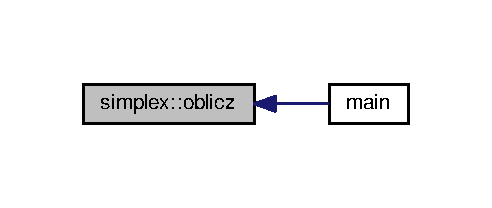
\includegraphics[width=236pt]{classsimplex_a6b34466c3336fa38ac333b9fbcfe26f4_icgraph}
\end{center}
\end{figure}


\hypertarget{classsimplex_a49d8689f9b244ffd9d1941dcc5382278}{\index{simplex@{simplex}!wprowadz\-\_\-dane@{wprowadz\-\_\-dane}}
\index{wprowadz\-\_\-dane@{wprowadz\-\_\-dane}!simplex@{simplex}}
\subsubsection[{wprowadz\-\_\-dane}]{\setlength{\rightskip}{0pt plus 5cm}void simplex\-::wprowadz\-\_\-dane (
\begin{DoxyParamCaption}
{}
\end{DoxyParamCaption}
)}}\label{classsimplex_a49d8689f9b244ffd9d1941dcc5382278}


Funkcja do wprowadzania danych. 

Dzialanie funkcji\-: -\/$>$ wpisanie ilosci rownan -\/$>$ wpisanie poszczegolnych wspolczynnikow -\/$>$ wpisanie poszczegolnych ograniczen -\/$>$ wpisanie poszczegolnych kosztow 

Definition at line 23 of file simplex.\-cpp.



Here is the caller graph for this function\-:\nopagebreak
\begin{figure}[H]
\begin{center}
\leavevmode
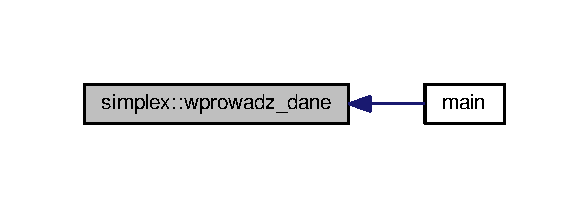
\includegraphics[width=282pt]{classsimplex_a49d8689f9b244ffd9d1941dcc5382278_icgraph}
\end{center}
\end{figure}


\hypertarget{classsimplex_a38765e9873e84c9c1574528d39f5e9d9}{\index{simplex@{simplex}!wyswietl@{wyswietl}}
\index{wyswietl@{wyswietl}!simplex@{simplex}}
\subsubsection[{wyswietl}]{\setlength{\rightskip}{0pt plus 5cm}void simplex\-::wyswietl (
\begin{DoxyParamCaption}
{}
\end{DoxyParamCaption}
)}}\label{classsimplex_a38765e9873e84c9c1574528d39f5e9d9}


Funkcja wyswietaljaca uklad rownan. 

Dzialanie funkcji\-: -\/$>$ wyswietlenie wynikow \-:
\begin{DoxyItemize}
\item zmienne z wspolczynikami
\item oraniczenia dla danego rownania 
\end{DoxyItemize}

Definition at line 57 of file simplex.\-cpp.



Here is the caller graph for this function\-:\nopagebreak
\begin{figure}[H]
\begin{center}
\leavevmode
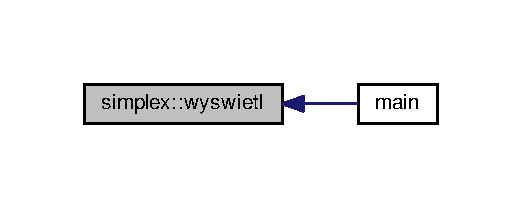
\includegraphics[width=250pt]{classsimplex_a38765e9873e84c9c1574528d39f5e9d9_icgraph}
\end{center}
\end{figure}




\subsection{Member Data Documentation}
\hypertarget{classsimplex_adfd1d227f38ea360def13b1f15b20939}{\index{simplex@{simplex}!koszt@{koszt}}
\index{koszt@{koszt}!simplex@{simplex}}
\subsubsection[{koszt}]{\setlength{\rightskip}{0pt plus 5cm}int simplex\-::koszt\mbox{[}2\mbox{]}\hspace{0.3cm}{\ttfamily [private]}}}\label{classsimplex_adfd1d227f38ea360def13b1f15b20939}


Pole typu int, bedzie uzywane do przechowywania kosztow 2och zmiennych. 



Definition at line 33 of file simplex.\-hh.

\hypertarget{classsimplex_a2345d5a390dc5284e4ed37d5f63ca5e8}{\index{simplex@{simplex}!n@{n}}
\index{n@{n}!simplex@{simplex}}
\subsubsection[{n}]{\setlength{\rightskip}{0pt plus 5cm}int simplex\-::n\hspace{0.3cm}{\ttfamily [private]}}}\label{classsimplex_a2345d5a390dc5284e4ed37d5f63ca5e8}


Pole typu int, bedzie uzywane do przechowywania ilosci rownan. 



Definition at line 41 of file simplex.\-hh.

\hypertarget{classsimplex_a8a31528b6dcde5dadf732e403f2910d1}{\index{simplex@{simplex}!ograniczenia@{ograniczenia}}
\index{ograniczenia@{ograniczenia}!simplex@{simplex}}
\subsubsection[{ograniczenia}]{\setlength{\rightskip}{0pt plus 5cm}double$\ast$ simplex\-::ograniczenia\hspace{0.3cm}{\ttfamily [private]}}}\label{classsimplex_a8a31528b6dcde5dadf732e403f2910d1}


Pole typu $\ast$double, bedzie uzywane do przechowywania ograniczen poszczegolnych rowan. 



Definition at line 29 of file simplex.\-hh.

\hypertarget{classsimplex_ac8767985af04610b7cbb310bb22a6f7c}{\index{simplex@{simplex}!tab@{tab}}
\index{tab@{tab}!simplex@{simplex}}
\subsubsection[{tab}]{\setlength{\rightskip}{0pt plus 5cm}double$\ast$$\ast$ simplex\-::tab\hspace{0.3cm}{\ttfamily [private]}}}\label{classsimplex_ac8767985af04610b7cbb310bb22a6f7c}


Pole typu $\ast$$\ast$double, bedzie uzywane do przechowywania macierzy ukladu rownan. 



Definition at line 25 of file simplex.\-hh.

\hypertarget{classsimplex_ac0619d7747a373ff01bf3dab3126b330}{\index{simplex@{simplex}!x@{x}}
\index{x@{x}!simplex@{simplex}}
\subsubsection[{x}]{\setlength{\rightskip}{0pt plus 5cm}double simplex\-::x\mbox{[}4\mbox{]}\hspace{0.3cm}{\ttfamily [private]}}}\label{classsimplex_ac0619d7747a373ff01bf3dab3126b330}


Definition at line 45 of file simplex.\-hh.

\hypertarget{classsimplex_abebe4828ea993bcfdb436a39123ce2c8}{\index{simplex@{simplex}!y@{y}}
\index{y@{y}!simplex@{simplex}}
\subsubsection[{y}]{\setlength{\rightskip}{0pt plus 5cm}double simplex\-::y\mbox{[}4\mbox{]}\hspace{0.3cm}{\ttfamily [private]}}}\label{classsimplex_abebe4828ea993bcfdb436a39123ce2c8}


Pola typu double, beda uzywane do zapisywania pozycji kluczowych punktow. 



Definition at line 45 of file simplex.\-hh.

\hypertarget{classsimplex_a08631fd56f6f55fb022860ee5edcbdf4}{\index{simplex@{simplex}!zysk@{zysk}}
\index{zysk@{zysk}!simplex@{simplex}}
\subsubsection[{zysk}]{\setlength{\rightskip}{0pt plus 5cm}double simplex\-::zysk\mbox{[}7\mbox{]}\hspace{0.3cm}{\ttfamily [private]}}}\label{classsimplex_a08631fd56f6f55fb022860ee5edcbdf4}


Pole typu double, bedzie uzywane do liczenia najlepszego zysku. 



Definition at line 37 of file simplex.\-hh.



The documentation for this class was generated from the following files\-:\begin{DoxyCompactItemize}
\item 
/home/pawel/\-Dokumenty/programowanie/pamsi/simplex/prj/inc/\hyperlink{simplex_8hh}{simplex.\-hh}\item 
/home/pawel/\-Dokumenty/programowanie/pamsi/simplex/prj/src/\hyperlink{simplex_8cpp}{simplex.\-cpp}\end{DoxyCompactItemize}

\chapter{File Documentation}
\hypertarget{strona_8dox}{\section{/home/pawel/\-Dokumenty/programowanie/pamsi/sortowanie/prj/doc/pages/strona.dox File Reference}
\label{strona_8dox}\index{/home/pawel/\-Dokumenty/programowanie/pamsi/sortowanie/prj/doc/pages/strona.\-dox@{/home/pawel/\-Dokumenty/programowanie/pamsi/sortowanie/prj/doc/pages/strona.\-dox}}
}

\hypertarget{simplex_8hh}{\section{/home/pawel/\-Dokumenty/programowanie/pamsi/simplex/prj/inc/simplex.hh File Reference}
\label{simplex_8hh}\index{/home/pawel/\-Dokumenty/programowanie/pamsi/simplex/prj/inc/simplex.\-hh@{/home/pawel/\-Dokumenty/programowanie/pamsi/simplex/prj/inc/simplex.\-hh}}
}


Definicje funkcji dla klasy simplex.  


{\ttfamily \#include $<$iostream$>$}\\*
Include dependency graph for simplex.\-hh\-:\nopagebreak
\begin{figure}[H]
\begin{center}
\leavevmode
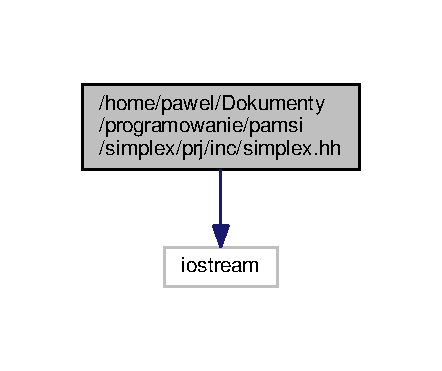
\includegraphics[width=212pt]{simplex_8hh__incl}
\end{center}
\end{figure}
This graph shows which files directly or indirectly include this file\-:\nopagebreak
\begin{figure}[H]
\begin{center}
\leavevmode
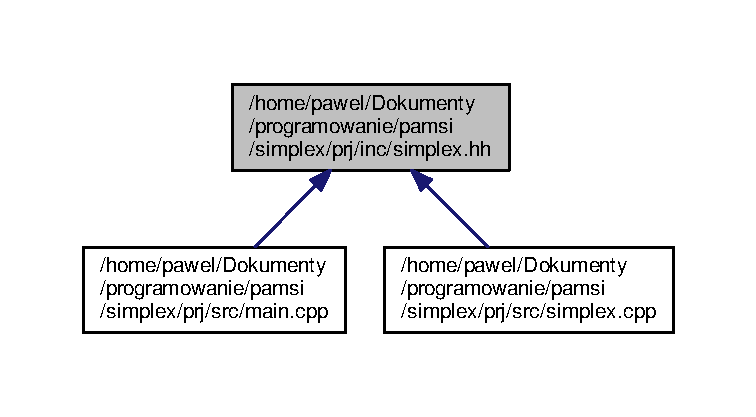
\includegraphics[width=350pt]{simplex_8hh__dep__incl}
\end{center}
\end{figure}
\subsection*{Classes}
\begin{DoxyCompactItemize}
\item 
class \hyperlink{classsimplex}{simplex}
\begin{DoxyCompactList}\small\item\em Modeluje pojecie Simplex. Klasa sluzy do wykonania uprostrzonego algorytmu simplex tzn \-: -\/$>$ znalezienia najwiekszego zysku z funkcji celu. \end{DoxyCompactList}\end{DoxyCompactItemize}


\subsection{Detailed Description}
Definicje funkcji dla klasy simplex. 

Definition in file \hyperlink{simplex_8hh_source}{simplex.\-hh}.


\hypertarget{main_8cpp}{\section{/home/pawel/\-Dokumenty/programowanie/pamsi/simplex/prj/src/main.cpp File Reference}
\label{main_8cpp}\index{/home/pawel/\-Dokumenty/programowanie/pamsi/simplex/prj/src/main.\-cpp@{/home/pawel/\-Dokumenty/programowanie/pamsi/simplex/prj/src/main.\-cpp}}
}


Plik zawiera funkcje \hyperlink{main_8cpp_ae66f6b31b5ad750f1fe042a706a4e3d4}{main()}  


{\ttfamily \#include $<$iostream$>$}\\*
{\ttfamily \#include \char`\"{}../inc/simplex.\-hh\char`\"{}}\\*
Include dependency graph for main.\-cpp\-:\nopagebreak
\begin{figure}[H]
\begin{center}
\leavevmode
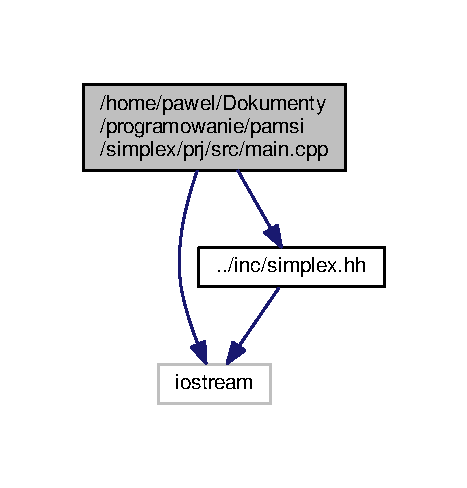
\includegraphics[width=224pt]{main_8cpp__incl}
\end{center}
\end{figure}
\subsection*{Functions}
\begin{DoxyCompactItemize}
\item 
int \hyperlink{main_8cpp_ae66f6b31b5ad750f1fe042a706a4e3d4}{main} ()
\end{DoxyCompactItemize}


\subsection{Detailed Description}
Plik zawiera funkcje \hyperlink{main_8cpp_ae66f6b31b5ad750f1fe042a706a4e3d4}{main()} 

Definition in file \hyperlink{main_8cpp_source}{main.\-cpp}.



\subsection{Function Documentation}
\hypertarget{main_8cpp_ae66f6b31b5ad750f1fe042a706a4e3d4}{\index{main.\-cpp@{main.\-cpp}!main@{main}}
\index{main@{main}!main.cpp@{main.\-cpp}}
\subsubsection[{main}]{\setlength{\rightskip}{0pt plus 5cm}int main (
\begin{DoxyParamCaption}
{}
\end{DoxyParamCaption}
)}}\label{main_8cpp_ae66f6b31b5ad750f1fe042a706a4e3d4}


Definition at line 13 of file main.\-cpp.



Here is the call graph for this function\-:\nopagebreak
\begin{figure}[H]
\begin{center}
\leavevmode
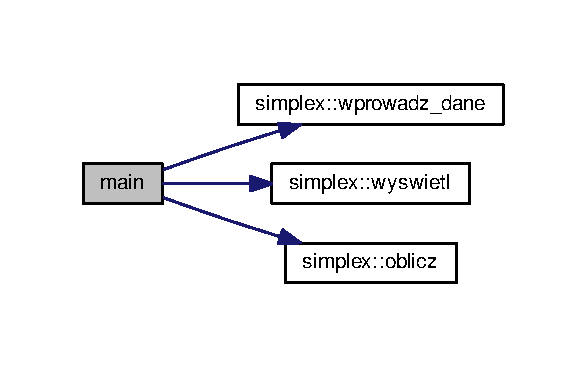
\includegraphics[width=282pt]{main_8cpp_ae66f6b31b5ad750f1fe042a706a4e3d4_cgraph}
\end{center}
\end{figure}



\hypertarget{simplex_8cpp}{\section{/home/pawel/\-Dokumenty/programowanie/pamsi/simplex/prj/src/simplex.cpp File Reference}
\label{simplex_8cpp}\index{/home/pawel/\-Dokumenty/programowanie/pamsi/simplex/prj/src/simplex.\-cpp@{/home/pawel/\-Dokumenty/programowanie/pamsi/simplex/prj/src/simplex.\-cpp}}
}


Plik zawiera funkcje z klasy simplex.  


{\ttfamily \#include \char`\"{}../inc/simplex.\-hh\char`\"{}}\\*
Include dependency graph for simplex.\-cpp\-:\nopagebreak
\begin{figure}[H]
\begin{center}
\leavevmode
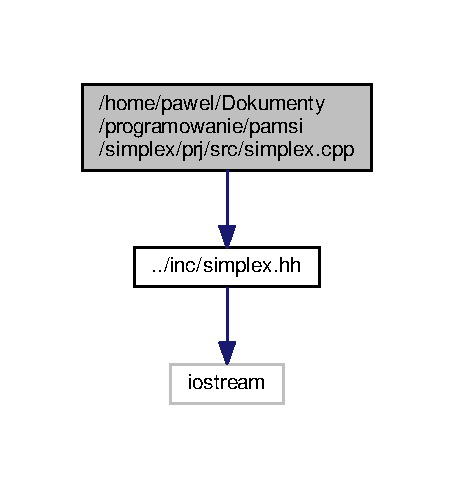
\includegraphics[width=218pt]{simplex_8cpp__incl}
\end{center}
\end{figure}


\subsection{Detailed Description}
Plik zawiera funkcje z klasy simplex. 

Definition in file \hyperlink{simplex_8cpp_source}{simplex.\-cpp}.


%--- End generated contents ---

% Index
\newpage
\phantomsection
\addcontentsline{toc}{chapter}{Index}
\printindex

\end{document}
